% Created by tikzDevice version 0.12.6 on 2024-06-12 14:46:42
% !TEX encoding = UTF-8 Unicode
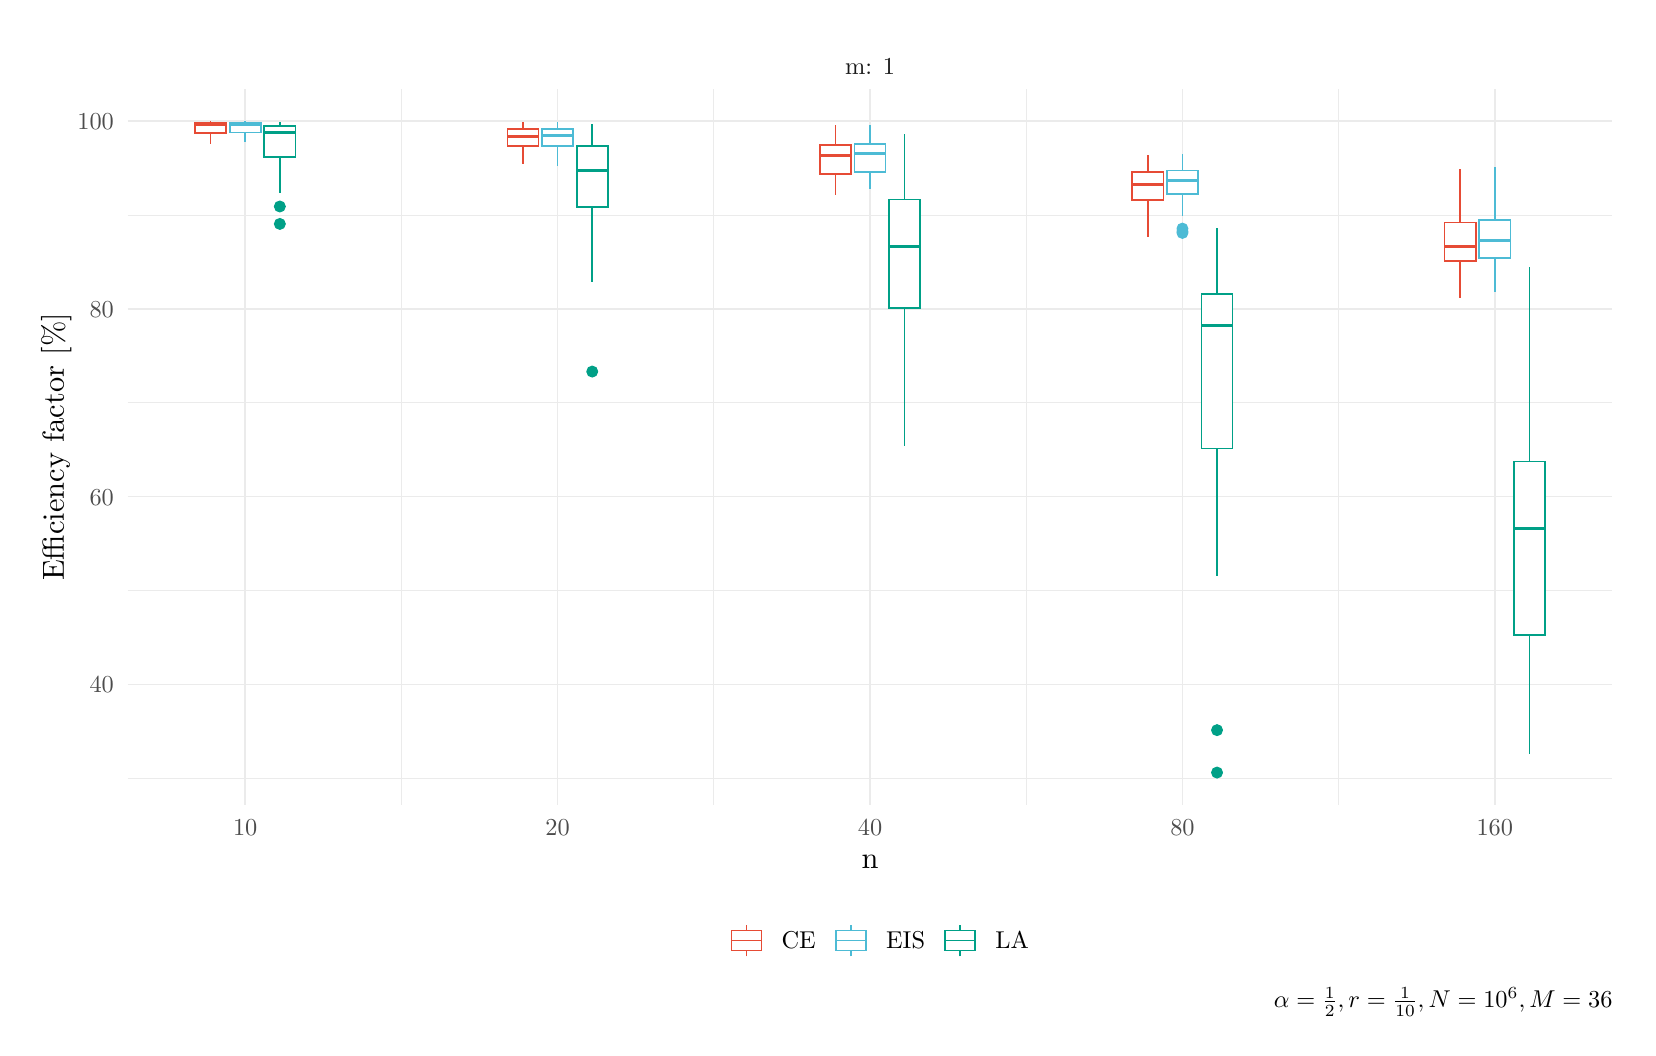
\begin{tikzpicture}[x=1pt,y=1pt]
\definecolor{fillColor}{RGB}{255,255,255}
\path[use as bounding box,fill=fillColor,fill opacity=0.00] (0,0) rectangle (578.16,361.35);
\begin{scope}
\path[clip] ( 36.11, 80.41) rectangle (572.66,339.28);
\definecolor{drawColor}{gray}{0.92}

\path[draw=drawColor,line width= 0.3pt,line join=round] ( 36.11, 90.15) --
	(572.66, 90.15);

\path[draw=drawColor,line width= 0.3pt,line join=round] ( 36.11,157.98) --
	(572.66,157.98);

\path[draw=drawColor,line width= 0.3pt,line join=round] ( 36.11,225.80) --
	(572.66,225.80);

\path[draw=drawColor,line width= 0.3pt,line join=round] ( 36.11,293.63) --
	(572.66,293.63);

\path[draw=drawColor,line width= 0.3pt,line join=round] (135.06, 80.41) --
	(135.06,339.28);

\path[draw=drawColor,line width= 0.3pt,line join=round] (247.95, 80.41) --
	(247.95,339.28);

\path[draw=drawColor,line width= 0.3pt,line join=round] (360.83, 80.41) --
	(360.83,339.28);

\path[draw=drawColor,line width= 0.3pt,line join=round] (473.71, 80.41) --
	(473.71,339.28);

\path[draw=drawColor,line width= 0.6pt,line join=round] ( 36.11,124.06) --
	(572.66,124.06);

\path[draw=drawColor,line width= 0.6pt,line join=round] ( 36.11,191.89) --
	(572.66,191.89);

\path[draw=drawColor,line width= 0.6pt,line join=round] ( 36.11,259.71) --
	(572.66,259.71);

\path[draw=drawColor,line width= 0.6pt,line join=round] ( 36.11,327.54) --
	(572.66,327.54);

\path[draw=drawColor,line width= 0.6pt,line join=round] ( 78.62, 80.41) --
	( 78.62,339.28);

\path[draw=drawColor,line width= 0.6pt,line join=round] (191.50, 80.41) --
	(191.50,339.28);

\path[draw=drawColor,line width= 0.6pt,line join=round] (304.39, 80.41) --
	(304.39,339.28);

\path[draw=drawColor,line width= 0.6pt,line join=round] (417.27, 80.41) --
	(417.27,339.28);

\path[draw=drawColor,line width= 0.6pt,line join=round] (530.15, 80.41) --
	(530.15,339.28);
\definecolor{drawColor}{RGB}{230,75,53}

\path[draw=drawColor,line width= 0.6pt,line join=round] ( 66.12,326.97) -- ( 66.12,327.50);

\path[draw=drawColor,line width= 0.6pt,line join=round] ( 66.12,323.37) -- ( 66.12,319.28);
\definecolor{fillColor}{RGB}{255,255,255}

\path[draw=drawColor,line width= 0.6pt,fill=fillColor] ( 60.50,326.97) --
	( 60.50,323.37) --
	( 71.75,323.37) --
	( 71.75,326.97) --
	( 60.50,326.97) --
	cycle;

\path[draw=drawColor,line width= 1.1pt] ( 60.50,326.22) -- ( 71.75,326.22);

\path[draw=drawColor,line width= 0.6pt,line join=round] (179.01,324.79) -- (179.01,327.26);

\path[draw=drawColor,line width= 0.6pt,line join=round] (179.01,318.50) -- (179.01,312.15);

\path[draw=drawColor,line width= 0.6pt,fill=fillColor] (173.38,324.79) --
	(173.38,318.50) --
	(184.63,318.50) --
	(184.63,324.79) --
	(173.38,324.79) --
	cycle;

\path[draw=drawColor,line width= 1.1pt] (173.38,322.08) -- (184.63,322.08);

\path[draw=drawColor,line width= 0.6pt,line join=round] (291.89,319.03) -- (291.89,326.11);

\path[draw=drawColor,line width= 0.6pt,line join=round] (291.89,308.48) -- (291.89,300.86);

\path[draw=drawColor,line width= 0.6pt,fill=fillColor] (286.26,319.03) --
	(286.26,308.48) --
	(297.51,308.48) --
	(297.51,319.03) --
	(286.26,319.03) --
	cycle;

\path[draw=drawColor,line width= 1.1pt] (286.26,315.32) -- (297.51,315.32);

\path[draw=drawColor,line width= 0.6pt,line join=round] (404.77,309.23) -- (404.77,315.51);

\path[draw=drawColor,line width= 0.6pt,line join=round] (404.77,299.01) -- (404.77,285.58);

\path[draw=drawColor,line width= 0.6pt,fill=fillColor] (399.14,309.23) --
	(399.14,299.01) --
	(410.39,299.01) --
	(410.39,309.23) --
	(399.14,309.23) --
	cycle;

\path[draw=drawColor,line width= 1.1pt] (399.14,304.80) -- (410.39,304.80);

\path[draw=drawColor,line width= 0.6pt,line join=round] (517.65,290.94) -- (517.65,310.18);

\path[draw=drawColor,line width= 0.6pt,line join=round] (517.65,277.00) -- (517.65,263.69);

\path[draw=drawColor,line width= 0.6pt,fill=fillColor] (512.02,290.94) --
	(512.02,277.00) --
	(523.27,277.00) --
	(523.27,290.94) --
	(512.02,290.94) --
	cycle;

\path[draw=drawColor,line width= 1.1pt] (512.02,282.35) -- (523.27,282.35);
\definecolor{drawColor}{RGB}{77,187,213}

\path[draw=drawColor,line width= 0.6pt,line join=round] ( 78.62,326.98) -- ( 78.62,327.51);

\path[draw=drawColor,line width= 0.6pt,line join=round] ( 78.62,323.44) -- ( 78.62,320.06);

\path[draw=drawColor,line width= 0.6pt,fill=fillColor] ( 73.00,326.98) --
	( 73.00,323.44) --
	( 84.25,323.44) --
	( 84.25,326.98) --
	( 73.00,326.98) --
	cycle;

\path[draw=drawColor,line width= 1.1pt] ( 73.00,326.24) -- ( 84.25,326.24);

\path[draw=drawColor,line width= 0.6pt,line join=round] (191.50,324.85) -- (191.50,327.28);

\path[draw=drawColor,line width= 0.6pt,line join=round] (191.50,318.69) -- (191.50,311.48);

\path[draw=drawColor,line width= 0.6pt,fill=fillColor] (185.88,324.85) --
	(185.88,318.69) --
	(197.13,318.69) --
	(197.13,324.85) --
	(185.88,324.85) --
	cycle;

\path[draw=drawColor,line width= 1.1pt] (185.88,322.23) -- (197.13,322.23);

\path[draw=drawColor,line width= 0.6pt,line join=round] (304.39,319.27) -- (304.39,326.15);

\path[draw=drawColor,line width= 0.6pt,line join=round] (304.39,309.09) -- (304.39,302.98);

\path[draw=drawColor,line width= 0.6pt,fill=fillColor] (298.76,319.27) --
	(298.76,309.09) --
	(310.01,309.09) --
	(310.01,319.27) --
	(298.76,319.27) --
	cycle;

\path[draw=drawColor,line width= 1.1pt] (298.76,315.71) -- (310.01,315.71);
\definecolor{fillColor}{RGB}{77,187,213}

\path[draw=drawColor,line width= 0.4pt,line join=round,line cap=round,fill=fillColor] (417.27,287.18) circle (  1.96);

\path[draw=drawColor,line width= 0.4pt,line join=round,line cap=round,fill=fillColor] (417.27,287.73) circle (  1.96);

\path[draw=drawColor,line width= 0.4pt,line join=round,line cap=round,fill=fillColor] (417.27,288.74) circle (  1.96);

\path[draw=drawColor,line width= 0.6pt,line join=round] (417.27,309.68) -- (417.27,315.76);

\path[draw=drawColor,line width= 0.6pt,line join=round] (417.27,301.33) -- (417.27,293.27);
\definecolor{fillColor}{RGB}{255,255,255}

\path[draw=drawColor,line width= 0.6pt,fill=fillColor] (411.64,309.68) --
	(411.64,301.33) --
	(422.89,301.33) --
	(422.89,309.68) --
	(411.64,309.68) --
	cycle;

\path[draw=drawColor,line width= 1.1pt] (411.64,306.29) -- (422.89,306.29);

\path[draw=drawColor,line width= 0.6pt,line join=round] (530.15,291.92) -- (530.15,311.07);

\path[draw=drawColor,line width= 0.6pt,line join=round] (530.15,278.18) -- (530.15,265.93);

\path[draw=drawColor,line width= 0.6pt,fill=fillColor] (524.52,291.92) --
	(524.52,278.18) --
	(535.77,278.18) --
	(535.77,291.92) --
	(524.52,291.92) --
	cycle;

\path[draw=drawColor,line width= 1.1pt] (524.52,284.47) -- (535.77,284.47);
\definecolor{drawColor}{RGB}{0,160,135}
\definecolor{fillColor}{RGB}{0,160,135}

\path[draw=drawColor,line width= 0.4pt,line join=round,line cap=round,fill=fillColor] ( 91.12,290.43) circle (  1.96);

\path[draw=drawColor,line width= 0.4pt,line join=round,line cap=round,fill=fillColor] ( 91.12,296.73) circle (  1.96);

\path[draw=drawColor,line width= 0.6pt,line join=round] ( 91.12,325.81) -- ( 91.12,327.40);

\path[draw=drawColor,line width= 0.6pt,line join=round] ( 91.12,314.66) -- ( 91.12,301.58);
\definecolor{fillColor}{RGB}{255,255,255}

\path[draw=drawColor,line width= 0.6pt,fill=fillColor] ( 85.50,325.81) --
	( 85.50,314.66) --
	( 96.75,314.66) --
	( 96.75,325.81) --
	( 85.50,325.81) --
	cycle;

\path[draw=drawColor,line width= 1.1pt] ( 85.50,323.60) -- ( 96.75,323.60);
\definecolor{fillColor}{RGB}{0,160,135}

\path[draw=drawColor,line width= 0.4pt,line join=round,line cap=round,fill=fillColor] (204.00,237.08) circle (  1.96);

\path[draw=drawColor,line width= 0.6pt,line join=round] (204.00,318.53) -- (204.00,326.60);

\path[draw=drawColor,line width= 0.6pt,line join=round] (204.00,296.53) -- (204.00,269.41);
\definecolor{fillColor}{RGB}{255,255,255}

\path[draw=drawColor,line width= 0.6pt,fill=fillColor] (198.38,318.53) --
	(198.38,296.53) --
	(209.63,296.53) --
	(209.63,318.53) --
	(198.38,318.53) --
	cycle;

\path[draw=drawColor,line width= 1.1pt] (198.38,309.75) -- (209.63,309.75);

\path[draw=drawColor,line width= 0.6pt,line join=round] (316.88,299.31) -- (316.88,323.05);

\path[draw=drawColor,line width= 0.6pt,line join=round] (316.88,259.95) -- (316.88,210.19);

\path[draw=drawColor,line width= 0.6pt,fill=fillColor] (311.26,299.31) --
	(311.26,259.95) --
	(322.51,259.95) --
	(322.51,299.31) --
	(311.26,299.31) --
	cycle;

\path[draw=drawColor,line width= 1.1pt] (311.26,282.27) -- (322.51,282.27);
\definecolor{fillColor}{RGB}{0,160,135}

\path[draw=drawColor,line width= 0.4pt,line join=round,line cap=round,fill=fillColor] (429.77,107.51) circle (  1.96);

\path[draw=drawColor,line width= 0.4pt,line join=round,line cap=round,fill=fillColor] (429.77, 92.18) circle (  1.96);

\path[draw=drawColor,line width= 0.6pt,line join=round] (429.77,265.20) -- (429.77,288.99);

\path[draw=drawColor,line width= 0.6pt,line join=round] (429.77,209.25) -- (429.77,163.12);
\definecolor{fillColor}{RGB}{255,255,255}

\path[draw=drawColor,line width= 0.6pt,fill=fillColor] (424.14,265.20) --
	(424.14,209.25) --
	(435.39,209.25) --
	(435.39,265.20) --
	(424.14,265.20) --
	cycle;

\path[draw=drawColor,line width= 1.1pt] (424.14,253.80) -- (435.39,253.80);

\path[draw=drawColor,line width= 0.6pt,line join=round] (542.65,204.64) -- (542.65,275.01);

\path[draw=drawColor,line width= 0.6pt,line join=round] (542.65,141.95) -- (542.65, 98.71);

\path[draw=drawColor,line width= 0.6pt,fill=fillColor] (537.02,204.64) --
	(537.02,141.95) --
	(548.27,141.95) --
	(548.27,204.64) --
	(537.02,204.64) --
	cycle;

\path[draw=drawColor,line width= 1.1pt] (537.02,180.41) -- (548.27,180.41);
\end{scope}
\begin{scope}
\path[clip] ( 36.11,339.28) rectangle (572.66,355.85);
\definecolor{drawColor}{gray}{0.10}

\node[text=drawColor,anchor=base,inner sep=0pt, outer sep=0pt, scale=  0.88] at (304.39,344.53) {m: 1};
\end{scope}
\begin{scope}
\path[clip] (  0.00,  0.00) rectangle (578.16,361.35);
\definecolor{drawColor}{gray}{0.30}

\node[text=drawColor,anchor=base,inner sep=0pt, outer sep=0pt, scale=  0.88] at ( 78.62, 69.40) {10};

\node[text=drawColor,anchor=base,inner sep=0pt, outer sep=0pt, scale=  0.88] at (191.50, 69.40) {20};

\node[text=drawColor,anchor=base,inner sep=0pt, outer sep=0pt, scale=  0.88] at (304.39, 69.40) {40};

\node[text=drawColor,anchor=base,inner sep=0pt, outer sep=0pt, scale=  0.88] at (417.27, 69.40) {80};

\node[text=drawColor,anchor=base,inner sep=0pt, outer sep=0pt, scale=  0.88] at (530.15, 69.40) {160};
\end{scope}
\begin{scope}
\path[clip] (  0.00,  0.00) rectangle (578.16,361.35);
\definecolor{drawColor}{gray}{0.30}

\node[text=drawColor,anchor=base east,inner sep=0pt, outer sep=0pt, scale=  0.88] at ( 31.16,121.03) {40};

\node[text=drawColor,anchor=base east,inner sep=0pt, outer sep=0pt, scale=  0.88] at ( 31.16,188.86) {60};

\node[text=drawColor,anchor=base east,inner sep=0pt, outer sep=0pt, scale=  0.88] at ( 31.16,256.68) {80};

\node[text=drawColor,anchor=base east,inner sep=0pt, outer sep=0pt, scale=  0.88] at ( 31.16,324.51) {100};
\end{scope}
\begin{scope}
\path[clip] (  0.00,  0.00) rectangle (578.16,361.35);
\definecolor{drawColor}{RGB}{0,0,0}

\node[text=drawColor,anchor=base,inner sep=0pt, outer sep=0pt, scale=  1.10] at (304.39, 57.36) {n};
\end{scope}
\begin{scope}
\path[clip] (  0.00,  0.00) rectangle (578.16,361.35);
\definecolor{drawColor}{RGB}{0,0,0}

\node[text=drawColor,rotate= 90.00,anchor=base,inner sep=0pt, outer sep=0pt, scale=  1.10] at ( 13.08,209.84) {Efficiency factor [\%]};
\end{scope}
\begin{scope}
\path[clip] (  0.00,  0.00) rectangle (578.16,361.35);
\definecolor{drawColor}{RGB}{230,75,53}

\path[draw=drawColor,line width= 0.6pt] (259.69, 25.72) --
	(259.69, 27.88);

\path[draw=drawColor,line width= 0.6pt] (259.69, 35.11) --
	(259.69, 37.28);
\definecolor{fillColor}{RGB}{255,255,255}

\path[draw=drawColor,line width= 0.6pt,fill=fillColor] (254.27, 27.88) rectangle (265.11, 35.11);

\path[draw=drawColor,line width= 0.6pt] (254.27, 31.50) --
	(265.11, 31.50);
\end{scope}
\begin{scope}
\path[clip] (  0.00,  0.00) rectangle (578.16,361.35);
\definecolor{drawColor}{RGB}{77,187,213}

\path[draw=drawColor,line width= 0.6pt] (297.48, 25.72) --
	(297.48, 27.88);

\path[draw=drawColor,line width= 0.6pt] (297.48, 35.11) --
	(297.48, 37.28);
\definecolor{fillColor}{RGB}{255,255,255}

\path[draw=drawColor,line width= 0.6pt,fill=fillColor] (292.06, 27.88) rectangle (302.90, 35.11);

\path[draw=drawColor,line width= 0.6pt] (292.06, 31.50) --
	(302.90, 31.50);
\end{scope}
\begin{scope}
\path[clip] (  0.00,  0.00) rectangle (578.16,361.35);
\definecolor{drawColor}{RGB}{0,160,135}

\path[draw=drawColor,line width= 0.6pt] (336.99, 25.72) --
	(336.99, 27.88);

\path[draw=drawColor,line width= 0.6pt] (336.99, 35.11) --
	(336.99, 37.28);
\definecolor{fillColor}{RGB}{255,255,255}

\path[draw=drawColor,line width= 0.6pt,fill=fillColor] (331.57, 27.88) rectangle (342.41, 35.11);

\path[draw=drawColor,line width= 0.6pt] (331.57, 31.50) --
	(342.41, 31.50);
\end{scope}
\begin{scope}
\path[clip] (  0.00,  0.00) rectangle (578.16,361.35);
\definecolor{drawColor}{RGB}{0,0,0}

\node[text=drawColor,anchor=base west,inner sep=0pt, outer sep=0pt, scale=  0.88] at (272.41, 28.47) {CE};
\end{scope}
\begin{scope}
\path[clip] (  0.00,  0.00) rectangle (578.16,361.35);
\definecolor{drawColor}{RGB}{0,0,0}

\node[text=drawColor,anchor=base west,inner sep=0pt, outer sep=0pt, scale=  0.88] at (310.21, 28.47) {EIS};
\end{scope}
\begin{scope}
\path[clip] (  0.00,  0.00) rectangle (578.16,361.35);
\definecolor{drawColor}{RGB}{0,0,0}

\node[text=drawColor,anchor=base west,inner sep=0pt, outer sep=0pt, scale=  0.88] at (349.71, 28.47) {LA};
\end{scope}
\begin{scope}
\path[clip] (  0.00,  0.00) rectangle (578.16,361.35);
\definecolor{drawColor}{RGB}{0,0,0}

\node[text=drawColor,anchor=base east,inner sep=0pt, outer sep=0pt, scale=  0.88] at (572.66,  7.21) {$\alpha = \frac 1 2, r = \frac 1 {10}, N = 10^{ 6 }, M=36$};
\end{scope}
\end{tikzpicture}
